\section{Objetivo del capítulo}\label{sec:benchmark}
En este capítulo se introducen los resultados de la evaluación empírica para las implementaciones
prototípicas de las tres alternativas propuestas a lo largo del trabajo: \vanilla, \compresschain,
y finalmente \hashchain.
La idea de los experimentos realizados es determinar la cantidad de elementos que pueden ser
añadidos a la \setchain por segundo, de modo de evaluar las siguientes hipótesis:
% Write hypothesis
\begin{itemize}
	\item La implementación de \compresschain presenta mejor rendimiento que la de \vanilla.
	\item La implementación de \hashchain presenta mejor rendimiento que la de \compresschain.
\end{itemize}

\section{Configuración}
%
La evaluación fue ejecutada sobre una MacBook Pro con procesador Apple M2 Max
con 12 núcleos y 64GB de RAM.

%
Todas las implementaciones fueron escritas en Golang y residen en un único ejecutable, el cual se encarga
de inicializar los siguiente servicios.
\begin{itemize}
	\item Un nodo de Tendermint adjunto a una versión específica de la aplicación (la cual impelementa los métodos
	de la ABCI). Las versiones disponibles de la aplicación son: \vanilla, \compresschain, y \hashchain.
	La versión de \hashchain utilizada implementa la estrategia de consolidación de época actual.
	Todas estas versiones de la 
	aplicación necesitan de una base de datos persistente para alojar la \setchain en sí.
	\item Para \compresschain y \hashchain, un servidor \collector RPC. Este servidor se encarga de recibir transacciones,
	armar los lotes adecuados (siguiendo la lógica correspondiente), y difundirlos mediante comunicación con el nodo
	de Tendermint. Por su parte, el \hcollector también requiere una base de datos persistente para guardar el mapeo de
	hashes a lotes de elementos.
	\item Un cliente, el cual se encarga de leer e interpretar transacciones, y enviarlas (comunicándose con el nodo de
	Tendermint en la versión \vanilla, o con el \collector correspondiente en los otros casos). Cada cliente se comunica
	con un único nodo servidor.
\end{itemize}
Para las bases de datos persistentes se utilizó \textit{BadgerDB}\cite{db.badger}.
Para las funciones criptográficas se utilizó el paquete crypto de ethereum. 

%
Cada instancia fue empaquetada en un contenedor Docker con uso limitado a 6 núcleros y 32GB de RAM.
%
La cantidad de nodos utilizados varió según cada experimento.
%
Fue utilizada la herramienta Docker-Compose para iniciar y correr los contenedores necesarios,
y proveer una red entre ellos de manera sencilla.


\section{Experimentos}
El funcionamiento de los experimentos llevados a cabo sigue la lógica presentada a continuación.
%
En principio, se inician las \textit{N} instancias que correspondan, según la configuración del experimento.
%
Como ya se mencionó, las instancias involucran tanto el nodo de Tendermint, como el \collector (en caso de
ser necesario), y el cliente.
%

Una vez inicializados los \textit{N} contenedores, los clientes comienzan a procesar los elementos asignados a cada
uno y a invocar \<add> para enviarlos.
%
Cada proceso cliente hace las invocaciones \<add> en el servidor que reside en su mismo contenedor. 
%
Esto implica (indirectamente) comunicarse con el nodo de Tendermint en el caso de \vanilla, y
comunicarse con el \collector correspondiente en el caso de \compresschain o \hashchain.

Los experimentos funcionan en rondas.
%
Cada experimento ejecuta X rondas, de Y segundos cada una.
%
Los clientes envían elementos cada Z segundos.
%
Luego de cada ronda, cada cliente envía una petición \<get> para registrar cuántas épocas y cuántos
elementos fueron efectivamente añadidos a la \setchain.
%
Los distintos servidores pueden diferir en la respuesta (ya que algunos pueden encontrarse atrasados
respecto a otros), por lo que se realiza un promedio de estos valores.
%
De este modo se logra estimar la cantidad de elementos añadidos por segundo.

\subsection{Parámetros}
Tendermint posee diversos parámetros que pueden configurarse.
Por ejemplo, el tamaño de la mempool
(en cantidad de transacciones y en cantidad de bytes) o el tamaño del bloque.
El valor de dichos parámetros fue tomado de \cite{tendermint.design}.

\bigskip

Así, los parámetros que se modifican en los experimentos son los siguientes:
\begin{itemize}
	\item \texttt{n\_nodes}: cantidad de nodos corriendo
	\item \texttt{sleep\_time}: cantidad de tiempo que espera el cliente antes de añadir un nuevo elemento
	\item \texttt{collector\_size}: cantidad de transacciones que el correspondiente \collector aloja antes de generar
	un lote (no válido para \vanilla).
\end{itemize}
La idea es ajustar los valores de los parámetros \texttt{sleep\_time} y \texttt{collector\_size},
de modo de obtener, para una cantidad determinada de nodos en la red, la máxima cantidad de elementos que pueden ser
añadidos a la \setchain para \vanilla, \compresschain y \hashchain.
Es importante notar que la cantidad de elementos enviados y añadidos a la \setchain debe mantenerse constante a lo largo
de todas las rondas ejecutadas.


\subsection{Elementos}
% También se puede citar Arbitrum Nitro: A Second-Generation Optimistic Rollup
Los elementos utilizados por los procesos clientes durante los experimentos son transacciones provenientes
de Arbitrum~\cite{Kalodner2018Arbitrum}, una tecnología de tipo \textit{Optimistic Rollup}~\footnote{
Arbitrum es una cadena lateral que corre en paralelo a la red principal de Ethereum.
También conocida como una solución de escalabilidad de capa 2 (L2), Arbitrum mejora la velocidad de las transacciones así
como los costos en comparación a la red principal.
Arbitrum fue fundada en 2021 y es al momento una de las tecnologías de capa 2 más populares en el mercado.}.
%

La elección de las transacciones fue tomada priorizando que los experimentos sean fieles a un contexto
real, respetando el contenido de las transacciones.
%
Fueron descargadas utilizando las API de Alchemy y de Chainstack\footnote{Disponibles en \url{https://www.alchemy.com/} y \url{https://chainstack.com/},
respectivamente.}, las
cuales permiten conectarse directamente a un nodo específico de Arbitrum que es parte de la red,
de modo de interactuar con los datos en la cadena y hacer las peticiones necesrias para descargar las transacciones.

%
Al analizar el conjunto de transacciones descargadas (alrededor de X transacciones) se encontró que el tamaño de
estas presentaba algunos valores extremos hacia la derecha.
Es decir, mientras que la mediana rondaba los 350 bytes, y la desviación estándar los 600 bytes, los valores mínimos y máximos eran de
110 bytes y  50 mil bytes, respectivamente.
Por tal motivo se decidió remover los valores extremadamente altos.
Siguiendo los valores modelo presentados en \cite{tendermint.design}, se limitó a utilizar transacciones de hasta 1KB de tamaño.
De este modo, analizando aproximadamente 100 mil transacciones provenientes del conjunto de datos usado
durante los experimentos (solo transacciones de hasta 1KB de tamaño), se obtuvieron los siguientes resultados.
\begin{itemize}
	\item Mediana: 340 bytes
	\item Desviación estándar: 220 bytes
	\item Min: 110 bytes
	\item Max: 1024 bytes
\end{itemize}

\section{Resultados}

A continuación se presentan los resultados obtenidos al ejecutar los experimentos para las tres alternativas,
con redes de 4, 10 y 20 nodos.

\subsection{Comentarios generales}

La primera observación que se hizo al analizar los resultados obtenidos es que el ratio al que los clientes envían elementos
debe ser elegido de modo de no saturar la mempool.
Esto quiere decir que debe evitarse enviar elementos a la mempool más rápidamente de lo que los elementos pueden salir de ella.

Cuando un cliente invoca \<add> en un servidor cuya mempool está llena\footnote{Siguiendo los valores utilizados en
~\cite{tendermint.design} la mempool puede alojar hasta 5000 transacciones con un tamaño máximo total de 1GiB.},
el elemento es rechazado y el cliente recibe un error.
A su vez, cuando se recibe un error por mempool llena, el cliente espera una cierta cantidad de tiempo para intentar
nuevamente el envío del elemento.
Esto produce un degradamiento en el ratio de elementos enviados por segundo.

Por su parte, si a medida que pasan las rondas del experimento se envían cada vez menos elementos, menos elementos pueden ser
añadidos a la \setchain, generando también un degradamiento en la cantidad de elementos añadidos por segundo.

Es por esto que los resultados estables son aquellos que no llegan a saturar la mempool en ningún momento del
experimento. Con \textit{resultado estable} nos referimos a que la cantidad de elementos enviados por parte de
los clientes así como también la cantidad de elementos añadidos a la \setchain se mantiente similar en cada
una de las rondas. 

\subsection{\vanilla}
Los experimentos para \vanilla fueron los más sencillos de llevar a cabo debido a que, variando la cantidad de nodos,
el único parámetro que debía ajustarse era \texttt{sleep\_time}.

A modo de ejemplo, en la Figura~\ref{fig:elements_against_sleep_time} se muestra la cantidad de elementos enviados en promedio por nodo por segundo,
al variar el valor de \texttt{sleep\_time}, durante todas las rondas de un experimento con 4 nodos.
Allí se puede observar que no es posible enviar mucho más de 400 elementos por segundo, dado que incluso disminuyendo el tiempo
que se espera antes de volver a invocar \<add>, la cantidad de elementos enviados por segundo no aumenta.
Esto es porque justamente al mandar elementos con demasiada frecuencia, la mempool se satura y los elementos comienzan a ser
rechazados, lo que genera una degradación en el ratio de elementos enviados por segundo.

A su vez, es interesante notar que la cantidad de elementos enviados en cada caso no es proporcional a la variación del valor del
parámetro \texttt{sleep\_time}.
Esto se explica considerando el hecho de que la invocación de \<add> tarda un tiempo no despreciable en comparación con
los valores de \texttt{sleep\_time}.

\begin{figure}
	\centering
	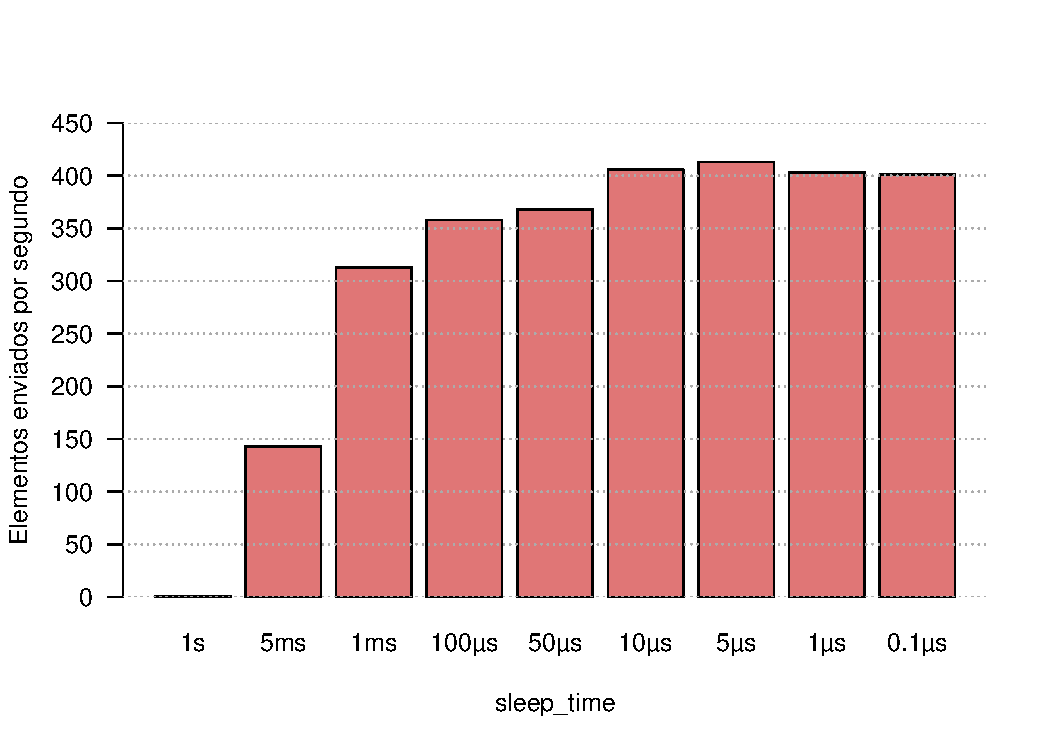
\includegraphics[scale=0.7]{figures/vanilla_4_nodos_elementos_enviados_segun_sleep.pdf}
	\caption{Promedio de elementos enviados por nodo variando \texttt{sleep\_time} en un experimento con 4 nodos para \vanilla.}
	\label{fig:elements_against_sleep_time}
\end{figure}

En la Figura~\ref{fig:vanilla_results} se muestra una comparación de la máxima cantidad de elementos añadidos en \vanilla para experimentos con
4, 10 y 20 nodos.
Se nota una clara degradación en la cantidad de elementos añadidos al aumentar la cantidad de nodos corriendo en el experimento.
Esta baja es esperable, sin embargo, es importante notar el siguiente punto.
Mientras más entidades (clientes y servidores) participen del consenso dentro de la red de Tendermint el experimento se hace más exigente en cuanto a recursos
(procesador y memoria RAM).
Dado que el límite de recursos destinados a Docker se mantiene constante durante todos los experimentos (independientemente de la cantidad de nodos),
se genera una degradación en la cantidad de elementos que los clientes pueden enviar por segundo.
Naturalmente, y como ya se mencionó antes, al disminuir el ratio de elementos enviados por segundo, invariablemente también lo hace el ratio de
elementos añadidos por segundo.

\begin{figure}
	\centering
	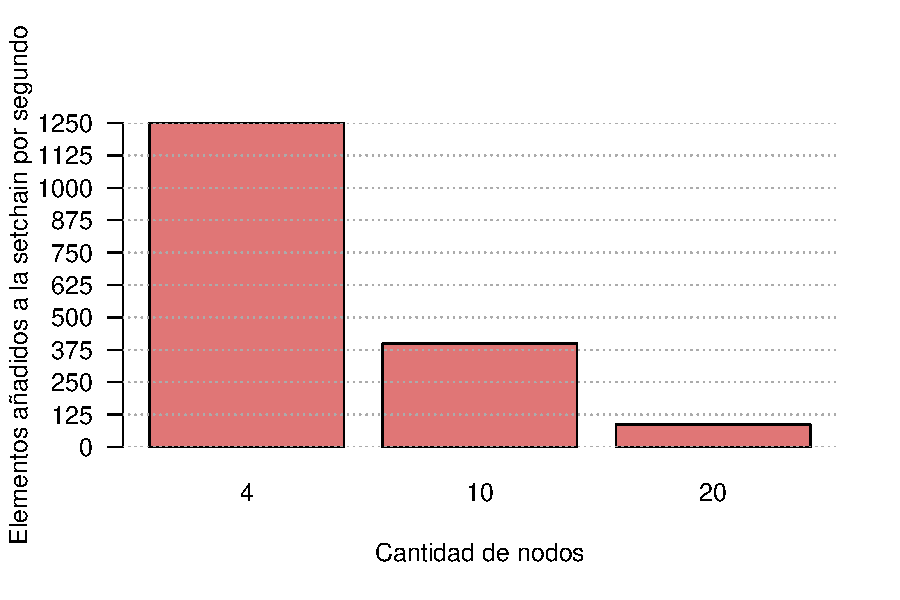
\includegraphics[scale=0.7]{figures/vanilla_resultados.pdf}
	\caption{Elementos añadidos a la \setchain por segundo según la cantidad de nodos para \vanilla.}
	\label{fig:vanilla_results}
\end{figure}
\subsection{\compresschain}
\subsection{\hashchain}
% \begin{itemize}
% 	\item Número de nodos: 4, 10, 100, 500, 1000, 2000
% 	\item Tamaño de collector: 800, 1000, 5000, 10000
% 	\item Sleep time: 5ms, 1ms, 100.000ns, 50.000ns, 10.000ns, 1.000ns
% \end{itemize}

% Primer experimento: bash config-benchmark.sh 4 /home/gabina/Tesina/localdeployment/txs/arbtxs /home/gabina/Tesina/localdeployment/setchain /home/gabina/Tesina/localdeployment/Dockerfile .


%%% Local Variables:
%%% TeX-master: "article.tex"
%%% TeX-PDF-mode: t
%%% End:
